\section{Sensors}\label{sec:sensors}

The sensor sub-system links directly to the user interface by providing plug-and-play functionality depending on mission requirements. Using modular sensors with standard interfaces and protocols, a wide variety of sensors can be fitted on the GVR-Bot. Power is provided through the vehicle's two BB-2590 batteries for up to 2 hours as the batteries each have 14 Ah, and with the full system operating, the current drain does not exceed 3A. The power system used for the prototype can support more power-draining sensors if required. The initial prototype can detect gases, liquids, and atmospheric conditions as shown in Fig.~\ref{fig:params}.

\begin{figure}[b]
	\centering
	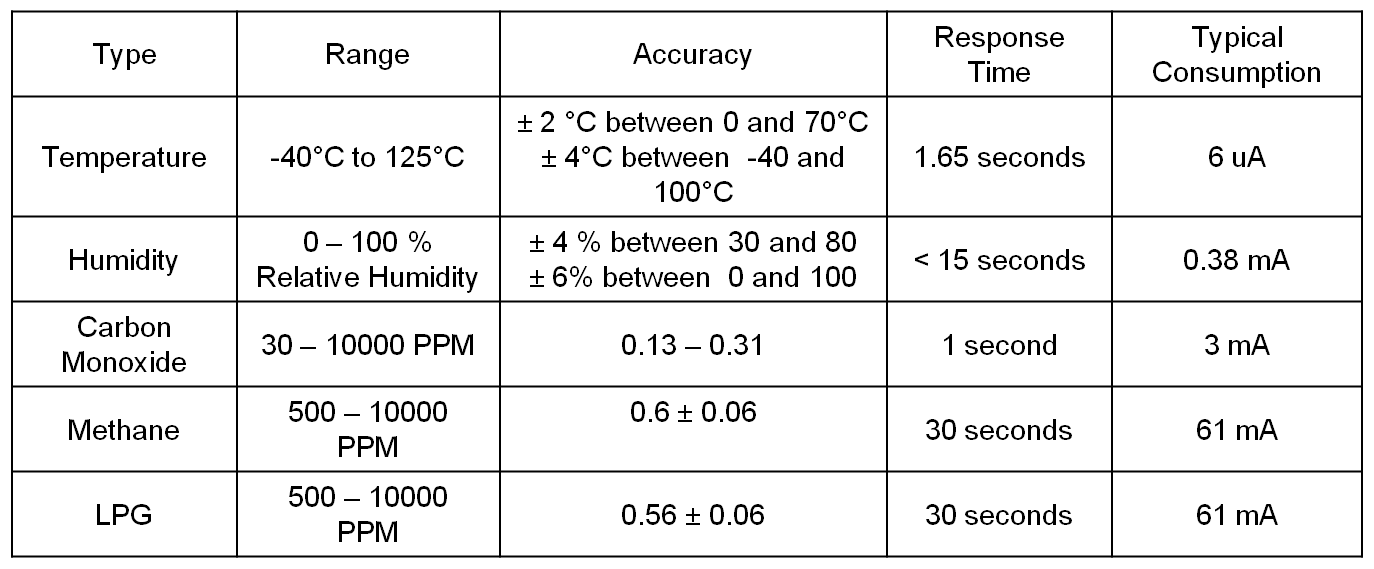
\includegraphics[width=0.48\textwidth]{./pictures/sensor_params.png}
	\caption{Types of sensors showing accuracy, response time, and power consumption rates.}
	\label{fig:params}
\end{figure}

For data acquisition, a microcontroller is used to process the sensor data and generate the data packets that are sent through the robot's embedded computer and wirelessly transmitted to the GUI to be stored in a database and displayed for the user. The software makes it possible for a user to modify, add, or subtract the current sensors used in order to fit the desired application. Furthermore, the multiple I/O channels on the microcontroller allow for easy access to integrate additional sensors. The structure of the sensor packet is scalable to add additional information as shown in Table \ref{tab:packet}. The received data is saved in a database to provide a history of the event readings. As explained in the user interface section, the familiarity of the GUI ensures that the user does not have to learn a completely new control interface. A sensor toolbar was developed to mesh with the robot's current user interface to provide live data readings. When a sensor reading passes a dangerous threshold, the toolbar will change colors to alert the operator. Under each sensor, a button displays a graph of the sensor's history.

\begin{table}
	\centering
	\begin{tabular}{ |l|l|l| }
		\hline
		\multicolumn{3}{ |c| }{Sensor Packet} \\
		\hline
		Sensor ID & Binary & 1 byte \\ \hline
		Data Type & Binary & 1 byte \\ \hline
		Data Length & Binary & 1 byte \\ \hline
		Data & (data type) & (data length) bytes \\
		\hline
	\end{tabular} 
	\caption{Sensor packet structure used to communicate sensor data back to the user interface.}
	\label{tab:packet}
\end{table}